



Human tissues are not easy to come by and 
We are interested in demixng RNA sequencing data (RNA-seq) that waseperating tissues
Unfortunately, there is no dataset that measure single cell profiles in the human brain. This posses a great challenge but also a great opportunity for blind-demixng. 
We use the brainspan dataset \cite{brainspan} to 
NMF since it is clear that using single cell profiles the profiles


We used brainspan data from K different region which was gathered from 8 humans subjects (we limit our anaylsis only to adult humans older than 17). There are ~8 samples from each region. Each expression is represtented by a vector of 52376 which hold sequnacing data both for coding region in the DNA and for noncoding regions. 

To evaluate the data we computed correlation between the reconstructed profiles and t
About the data




\begin{figure}[!hbt]
   (a) \hspace{120pt}(b) \hspace{120pt}(c) \hspace{120pt}
   \centering
     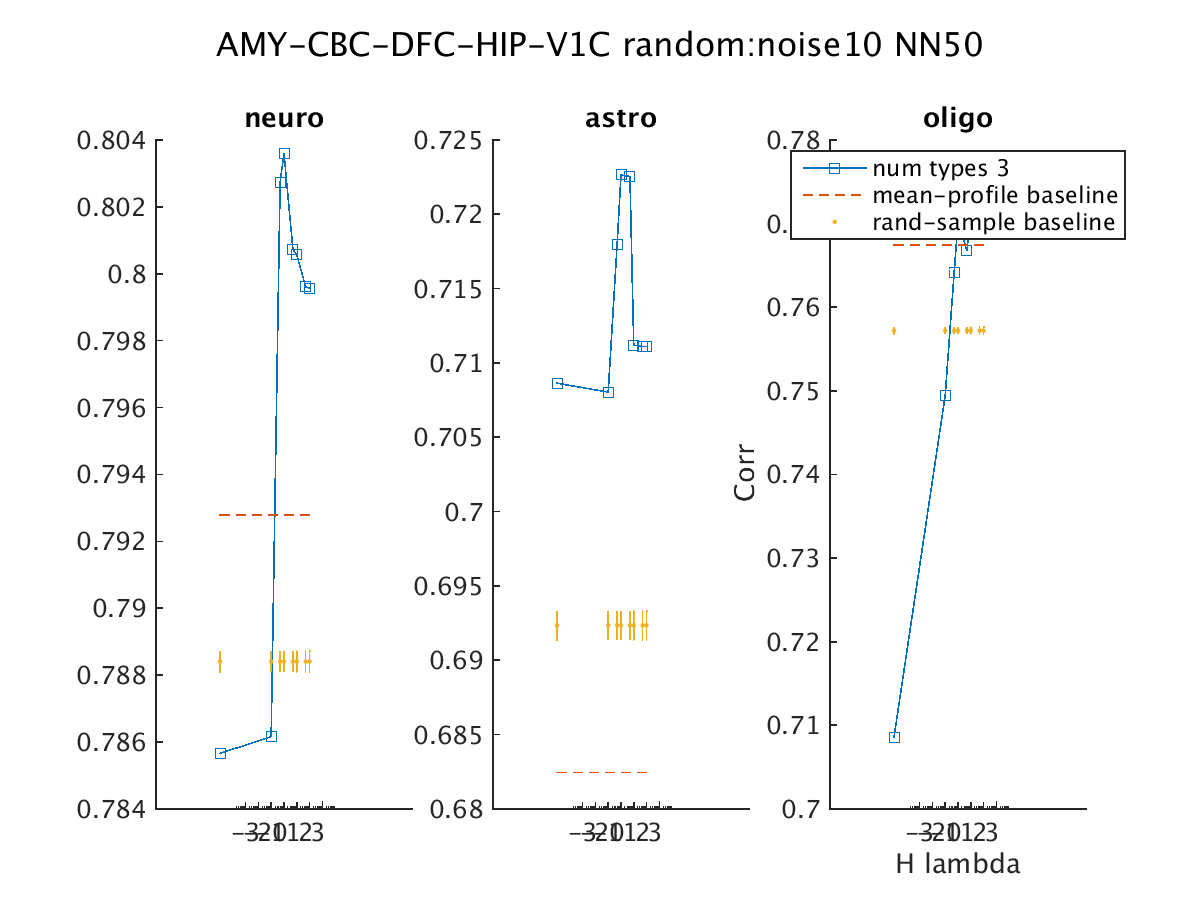
\includegraphics[width=0.95\textwidth]{human_data}
     caption{The effect of $\lambda$ on reconstruction}, 
    (a)  With a single region, all optimization method perform better as we introduced more samples. With a limited number of samples the active set and the block pivoting approaches performed the best. (b) Using multiple regions, the regularized connection between the region profiles help to reconstruct the original profiles. This is especially noticeable when only few samples are available for each region. (c) ????
    \label{fig:controlled_exp}
\end{figure}
